\documentclass[russian,utf8,nocolumnxxxi,nocolumnxxxii]{eskdtext}
\usepackage[T1,T2A]{fontenc}
\usepackage[utf8]{inputenc}
\usepackage[english,ukrainian,russian]{babel}
\usepackage{amsmath,amsfonts,amssymb,amsthm,mathtools} % AMS
\usepackage{icomma} % "Умная" запятая: $0,2$ --- число, $0, 2$ --- перечисление
%% Перенос знаков в формулах (по Львовскому)
%\newcommand*{\hm}[1]{#1\nobreak\discretionary{}
%{\hbox{$\mathsurround=0pt #1$}}{}}
\usepackage{cancel} % Для зачёркивания цифр
%%% Работа с картинками
\usepackage{graphicx}  % Для вставки рисунков
%\graphicspath{{images/}{images2/}}  % папки с картинками
%\setlength\fboxsep{3pt} % Отступ рамки \fbox{} от рисунка
%\setlength\fboxrule{1pt} % Толщина линий рамки \fbox{}
\usepackage{wrapfig} % Обтекание рисунков текстом
\usepackage{tikz}
\usepackage{pgfplots}
\usepackage{pgfplotstable}
\usepackage{siunitx}
\usepackage[american,cuteinductors,smartlabels]{circuitikz}
\usepackage[backend=biber]{biblatex}
\addbibresource{error_estimation_otchet.bib}
\usepackage[]{hyperref}
\hypersetup{
colorlinks=true,
}
\usepackage{textcomp}
\newcommand{\No}{\textnumero}
\ESKDdepartment{Федеральное агентство по образованию}
\ESKDcompany{Санкт-Петербургский государственный электротехнический университет "ЛЭТИ"}
\ESKDtitle{Пояснительная записка к Курсовой работе}
\ESKDsignature{Вариант N1}
\ESKDauthor{Авсюкевич С. В.}
\ESKDchecker{Прокшин~А.~Н.}
\ESKDdocName{по дисциплине "Информатика"}

\begin{document}

\begin{center}

Федеральное агентство по образованию

Санкт-Петербургский государственный

электротехнический университет "ЛЭТИ"

\end{center}

\vspace{8em}

\begin{center}
ПОЯСНИТЕЛЬНАЯ ЗАПИСКА К КУРСОВОЙ РАБОТЕ

по дисциплине "Информатика"

\end{center}

\vspace{2.5em}

\begin{center}

Вариант №1

\end{center}


\vspace{20em}

\begin{center}

2018

\end{center}
\newpage

\tableofcontents

\newpage
\section{Введение}

В настоящее время при решении различных как прикладных инженерных, так и чисто исследовательских задач, возникает необходимость в использовании широкого круга алгоритмов из множества разделов математики. Между тем самостоятельная реализация многих алгоритмов на некотором языке программирования может быть сложна и избыточна. Вследствие этого широкое распространение получили математические пакеты и системы компьютерной алгебры, такие как: MatLab, Octave, SciLab, Mathematica, Reduce, Mapple, призванные избавить пользователя от рутинных процедур, предоставить удобный интерфейс взаимодействия с уже написанным программным кодом и быстрым созданием нового. К сожалению, некоторые из перечисленных выше математических пакетов, будучи коммерческими по природе, имеют пакетом SciLab и системой компьютерной алгебры Reduce.

\newpage
 \subsection{Цель курсовой работы}
Ууметь применять персональный компьютер и математические пакеты прикладных программ в инженерной деятельности.
\subsection{Тема курсовой работы:}
Решение математических задач с использованием математического пакета «SciLab» и системы компьютерной алгебры «Reduce».

\subsection{Задание на курсавую работу}

\begin{enumerate}
\item Даны функции $f(x)=\sqrt{3}(x)+cos(x)$ и $g(x)=cos(2x+(\dfrac{\pi}{3})-1$
\begin{itemize}
  \item Решить уравнение f(x)=g(x)
  \item Исследовать функцию h(x)=f(x)-g(x) на промежутке $[0;\frac{5\pi}{6}]$
\end{itemize}
\item Найти коэффициенты кубического сплайна, интерполирующего данные, представленные в векторах $V_y$ и $V_x$.
\\Построить на графике функцию f(x), полученную после нахождения коэффициентов кубического сплайна.
\\Представить графическое изображение результатов интерполяции исходных данных различными методами с использованием встроенных функций.
\item Решить задачу оптимального распределения неоднородных ресурсов. На предприятии постоянно возникают задачи определения оптимального плана производства продукции при наличии конкретных ресурсов (сырья, полуфабрикатов, оборудования, финансов, рабочей силы и др.) или проблемы оптимизации распределения неоднородных ресурсов на производстве.
\\{\bfПостановка задачи.}  Для изготовления n видов изделий $N_1$, $N_2$, ..., $N_n$ необходимы ресурсы m видов: трудовые, материальные, финансовые и др. Известно требуемое количество отдельного i-гo ресурса для изготовления каждого j-го изделия. Назовем эту величину нормой расхода  $c_ij$. Пусть определено количество каждого вида ресурса, которым предприятие располагает в данный момент, - $a_i$. Известна прибыль $П_i$, получаемая предприятием от изготовления каждого j-го изделия. Требуется определить, какие изделия и в каком количестве должны производиться предприятием, чтобы прибыль была максимальной.
\end{enumerate}

%\begin{figure}[h]
%\begin{center}
%\includegraphics{Третье задание.jpg}}  
%\end{center}
%\end{figure}

\newpage

\section{Исследование функции}

Исследование функции — задача, заключающаяся в определении основных параметров заданной функции.

Даны функции $f(x)=\sqrt{3}sin(x)+cos(x),g(x)=cos(2x+\dfrac{\pi}{3})-1$
\begin{enumerate}
\item Решить уравнение $f(x)=g(x)$
\item Исследовать функцию $h(x)=f(x)-g(x)$ на промежутке $[0;\dfrac{5\pi}{6}]$
\end{enumerate}

\subsection{Решение уравнения}

Уравнение – это равенство, содержащее одно или несколько неизвестных, при условии, что ставится задача нахождения тех значений неизвестных, для которых оно истинно.

Решить уравнение – это значит найти все значения неизвестных, при которых оно обращается в верное числовое равенство, или установить, что таких значений нет.

Обычно при использовании мат. пакетов решение нелинейных уравнений можно получить двумя путями – численно и аналитически. Поскольку в «SciLab» и «SMath studio»  с помощью стандартных функций можно получить только численное решение, при нахождении аналитического воспользуемся системой компьютерной алгебры «Reduce».

\subsection{Аналетический метод решения}

Аналетический метод решения - это решение, представленное в виде формулы (и соответственно полученное тоже путём математических выкладок).

Для отыскания аналитического решения воспользуемся функцией solve из системы компьютерной алгебры «Reduce» где:
\begin{itemize}
 \item expr – список из уравнений (то есть система)
 \item var – список из переменных, относительно которых решаются уравнения expr
\end{itemize}

При попытке разрешить уравнение h(x)= 0 относительно x:\\
solve(sqrt(3)sin(x)+cos(x)-cos(2x+pi/3)-1,x);\\
получаем:

$$
\left\{x=root_{-}of\left(cos\left(\frac{6x_{-}+\pi}{3}\right)-cos(x_{-})-sqrt(3)sin(x_{-})-1, x_{-}, tag_{-2}\right)\right\}
$$

То есть решение данного уравнения не было найдено.
Упростим данное уравнение, воспользовавшись двумя тригонометрическими тождествами: 
\begin{align}
sin(x+y)=& sin(x)cos(y)+cos(x)sin(y)\\
cos(2x)=&1-2sin^2(x) 
\end{align}

Выразим множетели функции $f(x)$ таким образом:
\begin{align*}
\sqrt3=&2 cos\frac{\pi}{6},\\   
1=&2 sin\frac{\pi}{6}
\end{align*}

Функцию $f(x)=\sqrt3 sin(x)+cos(x)$ запишем так:
\begin{align*}
sin(x) \times 2 &cos(\frac{\pi}{6})+cos(x) \times 2 sin(\frac{\pi}{6})\\
2\times(sin(x)\times &cos(\frac{\pi}{6})+cos(x) \times sin(\frac{\pi}{6}))\\
2& sin(x+\frac{\pi}{6})
\end{align*}

Функцию $g(x)=cos(2x+\frac{\pi}{3})-1$ запишим так:
\begin{align*}
\cancel{1}-2sin^2&(x+\frac{\pi}{6})-\cancel{1}\\
2sin^2&(x+\frac{\pi}{6})
\end{align*}



И получим тривиальное уравнение, эквивалентное исходному
$$2(sin(x+\frac{\pi}{6})+sin^2(x+\frac{\pi}{6}))=0$$

Применим к нему функцию solve в программе "Reduce":\\
solve(2sin(x+pi/6)*(1+sin(x+pi/6)));
и получим решение:

\begin{align*}
	x=&\frac{\pi(arbint(4)+5)}{6},& x=&\frac{\pi(12arbint(4)-1)}{6},\\ 
x=&\frac{2\pi(arbint(3)+2)}{3},& x=&\frac{2\pi(3arbint(3)-1)}{3} 
\end{align*}

где arbint (arbitrary integer) является произвольным целым числом. Запишем решение в более привычной форме:

$$x_1=\frac{5}{6}*\pi+2n\pi,n\in Z$$
$$x_2=-\frac{1}{6}*\pi+2n\pi,n\in Z$$
$$x_3=\frac{8}{6}*\pi+2n\pi,n\in Z$$
$$x_4=-\frac{4}{6}*\pi+2n\pi,n\in Z$$\\

Периодические решения для $x_3$ и $x_4$ совпадают, а периодическое решение для $x_2$ можно записать в виде:
$$x_2=\frac{11}{6}*\pi+2n\pi,n\in Z$$

Таким образов воспользовавшись математическим пакетом «Reduce» мы получили ответ Аналетическим способом. Но для более полн	 картины мы должны найти корни и Числовым методом используя пакет«SMath studio».

\subsection{Числовой метод решения} \label{resh}

Для отыскания численного решения воспользуемся стандартной функцией «SMath studio» solve.

«SMath studio» позволяет находить корни уравнения (нуля функции), т.е. точки, где значение функции равно нулю (графически пересекает ось X).Исследуем два выражения «$f(x)=\sqrt{3}sin(x)+cos(x),g(x)=cos(2x+\dfrac{\pi}{3})-1$». Из этого выражения можно построить функцию «$f(x)=\sqrt3 sin(x)+cos(x)-cos(2x+\frac{\pi}{3})+1$» 


В результате построения полкчился график изображённый на рисунке \ref{graf1}.
\begin{figure}[h]
\begin{center}
\begin{tikzpicture}
\begin{scope}[scale=1]

\draw[thin, ->] (-5,0) -- (5,0) node[right] {$X$};
\draw[thin, ->] (0,-3) -- (0,5) node[left] {$Y$};

%\foreach \x\xtext in{-1/-1,0.38/0.38,2/2,2.6/2.6,} %
%\draw (\x,0.1) -- (\x,-0.1) node[below] {$\xtext$}

%\draw[domain=-10:10, smooth, purple] plot ({\x},{(((sqrt(3))*(sin((\x))))+(cos((\x)))-(cos(2*(\x)+(pi\3)))+1)});
\draw[domain=-5:5, smooth, purple] plot ({\x},{(sqrt(3)*sin(\x r)+cos(\x r)-cos((2*(\x r))+(pi/3 r))+1)});
%\draw[domain=-5:5] plot ({\x},{((\x)*(\x))+2});

%\draw [domain=-10:10, smooth, green] plot ({(\x)},{sin(\x r)})


\end{scope}
\end{tikzpicture}
\caption{График функции $f(x)=\sqrt3 sin(x)+cos(x)-cos(2x+\frac{\pi}{3})+1$}
\label{graf1}
\end{center}
\end{figure}

Для того чтобы найти корни уравнения используем функции solve( ) с двумя аргументами (первый задаёт функцию, а второй переменную, по которой ведётся поиск корней), как и команда «Найти корни» , ищет корни в заданном в настройках диапазоне (Сервис/Опции/Вычисление/Корни/Диапазон), по умолчанию – 20..20. Выбираем диапазон - 5...5. 

В результате программа «SMath studio» выдала ответ:
\[
solve(f(x); x)=\begin{cases}
-3.6652\\
-0.5236\\
2.618
\end{casecs}
\]

Теперь мы можем указать эти значения на графике \ref{graf2} изображённом ниже.

\begin{figure}
\begin{center}
\begin{tikzpicture}
\begin{scope}[scale=1]

\draw[thin, ->] (-5,0) -- (5,0) node[right] {$X$};
\draw[thin, ->] (0,-3) -- (0,5) node[left] {$Y$};

\draw[domain=-5:5, smooth, purple] plot ({\x},{(sqrt(3)*sin(\x r)+cos(\x r)-cos((2*(\x r))+(pi/3 r))+1)});

\filldraw ( -3.6652, 0) circle (0.1cm) node [below=10pt] {-3.6652};
\filldraw (- 0.5236, 0) circle (0.1cm) node [below=20pt,left] {-0.5236};
\filldraw (2.618, 0) circle (0.1cm) node [below=20pt,right] {2.618};

\end{scope};
\end{tikzpicture}
\caption{График функции $f(x)$ с отмеченными корнями} \label{graf2}
\end{center}
\end{figure}

Таким образом видно, где находятся наши корни уравнения $f(x)$ на графике в интервале (-5, 5).

\subsection{Порядок исследования функции}

Алгаритм исследованиия функции:
\begin{enumerate}
 \item Найти область определения. Выделить особые точки (точки разрыва)
 \item Проверить наличие вертикальных асимптот в точках разрыва и на границах области определения
 \item Найти точки пересечения с осями координат
\item Установить, является ли функция чётной или нечётной
\item Определить, является ли функция периодической или нет (только для тригонометрических функций)
\item Найти точки экстремума и интервалы монотонности
\item Найти точки перегиба и интервалы выпуклости-вогнутости
\item Найти наклонные асимптоты. Исследовать поведение на бесконечности
\item Выбрать дополнительные точки и вычислить их координаты
\item Построить график и асимптоты.
\end{enumerate}

\subsubsection{Найти область определения. Выделить особые точки (точки разрыва)}

Данная функция имеет следующую область определения функции $ h(x)=\sqrt{3} sin(x)+cos(x)-cos(2x+\frac{\pi}{3})+1$: 
$$x\in R$$

%\subsubsection{Область возможных значений функции}

\subsubsection{Точки пересечения с осями координат}

Для того чтобы найти точки пересечения с осями необходимо вместо переменых подставить вместо премныых значение «0».

Находим точки пересечения с осью $О_x$. В разделе \ref{resh}  уже были найдены эти значения. 
$$
O_x: \text{точки } A(-3.6652, 0);  B( -0.5236, 0); C(2.618, 0).
$$

Находим точки пересечения с осью $O_y$. Для этого в программе «SMath studio» подставляем $x=0$ и получаем:
$$
O_y: \text{точка } D (0, 1.5)
$$

Точки пересечения функции ($h(x)$) с осями $O_x$ и $O_y$ представлены на рисунке \ref{graf3}.

По заданию необходимо исследовать функцию $h(x)$ на итервале $[o, \frac{5\pi}{6}]$ \Rightarrow в этот интервал попадает одна точка по оси $O_x$ равная $C(2.618,0)$ и точка $D(0, 1.5)$ с осью $O_y$. Данные точки представлены в соответстсвии с рисунком \ref{graf4}.


 \begin{figure}[h!]
\begin{center}
\begin{tikzpicture}
\begin{scope}[scale=1]

\draw[thin, ->] (-5,0) -- (5,0) node[right] {$X$};
\draw[thin, ->] (0,-3) -- (0,5) node[left] {$Y$};

\draw[domain=-5:5, smooth, purple] plot ({\x},{(sqrt(3)*sin(\x r)+cos(\x r)-cos((2*(\x r))+(pi/3 r))+1)});

\filldraw ( -3.6652, 0) circle (0.1cm) node [below=20pt,left=0.1cm] {$A(-3.6652,0)$};
\filldraw (- 0.5236, 0) circle (0.1cm) node [above=0.5cm,left] {$B(-0.5236, 0)$};
\filldraw (2.618, 0) circle (0.1cm) node [below=20pt,right] {$C(2.618, 0)$};
\filldraw (0, 1.5) circle (0.1cm) node [right] {$D(0, 1.5)$};
	
\end{scope};
\end{tikzpicture}
\caption{График функции $h(x)$ с точками пересечения осей $O_x$ и $O_y$} \label{graf3}
\end{center}
\end{figure}

\subsubsection{Анализ поиска вертикальной асимптоты}

По условию задания граничными точками области определения являются$(0;\frac{5\pi}{6})$

На границах области определения функция имеет вертикальные асимптоты, если односторонние пределы функции в этих граничных точках бесконечны.

Поскольку математический пакет "Scilab" не имеет возможности посчитать пределы, данную операцию пройдётся сделать частично в ручную.



Рассчитаем вертикальную асимптоту при х=0, точка является началом промежутка исследования функции h(x):

\begin{center}

$\lim\limits_{x\to{0-0}}\sqrt{3}sin(x)+cos(x)-cos(2x+\frac{\pi}{3})+1=\lim\limits_{x\to{0-0}}1.5\neq\pm\infty$

\end{center}

Из этого следует что по краю исследуемого промежутка вертикальных асимптот не наблюдается.
В момент расчётов в функцию h(x) было подставленною значение х в математический пакет "Scilab".

Листинг программы:
\\
\\$-->x=0$
\\ x  =
\\

\\$0.$
\\
\\$-->\sqrt(3)*sin(x)+cos(x)-cos((2*x) + ((pi)/3))+1$
\\ ans  =
\\

\\$1.5$

Рассчитаем вертикальную асимптоту при x=$\frac{5\pi}{6}$, точка является концом промежутка исследования функции h(x):

\begin{center}

$\lim\limits_{x\to{\frac{5\pi}{6}+0}}\sqrt{3}sin(x)+cos(x)-cos(2x+\frac{\pi}{3})+1=\lim\limits_{x\to{\frac{5\pi}{6}+0}}-2,22\neq\pm\infty$

\end{center}

Из этого следует что по краю исследуемого промежутка вертикальных асимптот не наблюдается.
В момент расчётов в функцию h(x) было подставленною значение х в математический пакет "Scilab".

Листинг программы:
\\
\\$-->x=(5*(pi))/6$
\\ x  =
//

 2.61
\\
\\$-->q=sqrt(3)*sin(x)+cos(x)-cos((2*x) + ((pi)/3))+1$
q  =

- 2.22

\subsubsection{Анализ выявления чётности, нечётности функции}

Из этого следует что при решении следует:
\[
\begin{center}
\begin{cases}
x=-1
\\
$h(-x) = \sqrt{3}sin(x)+cos(x)-cos(2x+\frac{\pi}{3})+1=- 0.0349609$
\end{cases}
\end{center}
\]\\
\[
\begin{center}
\begin{cases}
x=1
\\
$h(x) = ((\sqrt{3})*(sin(x))+(cos(x)))-((cos(2*x) + (\pi/3)) - 1)=- 0.0349609$
\end{cases}
\end{center}
\]
\\
\begin{center}
$h(-x) = h(-x) \Longleftrightarrow - 0.0349609 = - 0.0349609 \Longrightarrow$ Функция чётная.
\end{center}

Из этого следует что функция является симметричной.
В момент расчётов в функцию h(x) было подставленною значение х в математический пакет "Scilab" и использован следующий листинг:

$-->$x1=-1\\
 x1  =\\

  - 1.
 \\
$-->$q1=sqrt(3)*sin(x)+cos(x)-cos((2*x) + ((pi)/3)) + 1\\
 q1  =\\


         column 1 to 6\\

  - 0.0349609  - 0.0448128  - 0.0849485  - 0.1727211  - 0.3132469  - 0.4599841  \\

         column  7 to 12\\

  - 0.4817829  - 0.1877381    0.5573472    1.6851065    2.8831929    3.7428516  \\

         column 13 to 16\\

    3.9959654    3.6480703    2.9206719    2.0889372  \\

-->x2=1\\
 x2  =\\

    1.
\\
-->q2=sqrt(3)*sin(x)+cos(x)-cos((2*x) + ((pi)/3)) + 1\\
 q2  =
 \\
\\

         column 1 to 6\\

  - 0.0349609  - 0.0448128  - 0.0849485  - 0.1727211  - 0.3132469  - 0.4599841

         column  7 to 12\\

  - 0.4817829  - 0.1877381    0.5573472    1.6851065    2.8831929    3.7428516  \\

         column 13 to 16\\

    3.9959654    3.6480703    2.9206719    2.0889372 \\

-->if ( q1 == q2 ) then\\
-->disp ( "Чётная" )\\

 Чётная  \\
-->elseif ( q1 == (q2)*(-1) ) then\\
-->disp ( " Не чётная! " )\\
-->else\\
-->disp ( " В общем виде" )\\
-->end\\

\subsubsection{Построение графика y=h(x)}

Поскольку для упрощения поиска производных первого и второго порядков, значение которых максимально приближено к нулю, проще ориентироваться уже по готовому графику функции h(x), построение следует провести на данном этапе.

Для построения графика h(x) необходимо определить в каком пространстве находится данный график. Поскольку в исследуемой функции координата y выражается через координату x, данный график строиться в двухмерном пространстве. Для построения графика в двухмерном пространстве используются следующие команды в математическом пакете "Scilab".Команда plot которая предназначена для построения графика одной функции y = f (x). Обращение к ней имеет вид plot(x,y,[xcap,ycap,caption]) где x — массив абсцисс, y — массив ординат, xcap, ycap, caption — подписи осей X, Y и графика соответственно. Для создания функции y = f (x) используется команда function  f=y(x), f=x+a, endfunction;. Данная команда так же используется при получении производной первого и второго порядка методом приближения.

Пример листинга построения простейшего графика в математическом пакете "Scilab":
\\
-->function f = myquadratic ( x )\\
-->f = x+1\\
-->endfunction\\

-->xdata = linspace ( 0,3,200 );\\

-->ydata = myquadratic ( xdata );\\

-->plot ( xdata , ydata )\\

Результат построения графика представлен в соотвецтвии с рисунком \ref{graf4}.

 \begin{figure}[h!]
\begin{center}
\begin{tikzpicture}
\begin{scope}[scale=2]

\draw[thin, ->] (-1,0) -- (3.5,0) node[right] {$X$};
\draw[thin, ->] (0,-1) -- (0,4.5) node[left] {$Y$};

\draw[domain=0:2.7, smooth, purple] plot ({\x},{(sqrt(3)*sin(\x r)+cos(\x r)-cos((2*(\x r))+(pi/3 r))+1)});

%\filldraw ( -3.6652, 0) circle (0.1cm) node [below=20pt,left=0.1cm] {$A(-3.6652,0)$};
%\filldraw (- 0.5236, 0) circle (0.1cm) node [above=0.5cm,left] {$B(-0.5236, 0)$};
\filldraw (2.618, 0) circle (0.1cm) node [below=20pt,right] {$C(2.618, 0)$};
\filldraw (0, 1.5) circle (0.1cm) node [right] {$D(0, 1.5)$};
	
\end{scope};
\end{tikzpicture}
\caption{График функции $h(x)$ в пределах $[0, \frac{5\pi}{6}]} \label{graf4}
\end{center}
\end{figure}

\subsubsection{Производная первого и второго порядков с помощью интерполяционной формулы Ньютона.}

Данный способ заключается в том, что функцию y(x), заданную в равно стоящих точках $x_i$ отрезка [a,b] с помощью значений $y_1=f(x_i)$, приближенно заменяют интерполяционным полиномом Ньютона,  построенном для системы узлов $x_0,x_1,.....,x_k(k \leqslant n)$ и вычисляют производные $y'=f'(x), y''=f''(x)$.

Для выявления точки экстремума производная исследуемой функции должна быть равна нулю $h(x)=0$. При расчётах на исследуемый области $x=(0;\frac{5\pi}{6}$, ориентируясь по рисунку №2 видим что количество таких точек равно единице, поскольку поскольку функция в данном случае изгибается один раз.
Возьмём за первичную точку приближения, х=1. В следствии чего получим $h'(x)=0.2873079$. Поскольку приближение к нулю в десятых долях является достаточно большим, возьмём за точку приближения х=1,04. В следствии получим $h'(x)=0.0475615$. Приближение к нулю в погрешности сотых долей является малым, но не достаточно. возьмём за точку приближения х=1,048. В следствии получим $h'(x)=- 0.0004526$. Для максимального приближения к нулю используем х=1.047921. В следствии получим $h'(x)=0.0000215$. Данное приближение вполне можно считать допустимым.

Листин проводимых расчётов в математическом пакете "Scilab":\\
$-->$h=0.1;\\

$-->$x=1:h:(5*(pi)/6);\\

$-->$y=sqrt(3)*sin(x)+cos(x)-cos((2*x) + ((pi)/3)) + 1;\\

$-->$dy=diff(y);\\

$-->$dy2=diff(y,2);\\

$-->$dy3=diff(y,3);\\

$-->//$Приближенное значение y’(х)\\

$-->$Y=(dy(1)-dy2(1)/2+dy3(1)/3)/h\\
 Y  =\\

    0.2873079\\

$-->$h=0.1;\\

$-->$x=1.04:h:(5*(pi)/6);\\

$-->$y=sqrt(3)*sin(x)+cos(x)-cos((2*x) + ((pi)/3)) + 1;\\

$-->$dy=diff(y);\\

$-->$dy2=diff(y,2);\\

$-->$dy3=diff(y,3);\\

$-->//$Приближенное значение y’(х)\\

-1->Y=(dy(1)-dy2(1)/2+dy3(1)/3)/h\\
 Y  =\\

    0.0475615\\

$-->$h=0.1;\\

$-->$x=1.048:h:(5*(pi)/6);\\

$-->$y=sqrt(3)*sin(x)+cos(x)-cos((2*x) + ((pi)/3)) + 1;\\

$-->$dy=diff(y);\\

$-->$dy2=diff(y,2);\\

$-->$dy3=diff(y,3);\\

$-->//$Приближенное значение y’(х)\\

$-->$Y=(dy(1)-dy2(1)/2+dy3(1)/3)/h\\
 Y  =\\

  - 0.0004526\\

$-->$h=0.1;\\

$-->$x=1.047921:h:(5*(pi)/6);\\

$-->$y=sqrt(3)*sin(x)+cos(x)-cos((2*x) + ((pi)/3)) + 1;\\

$-->$dy=diff(y);\\

$-->$dy2=diff(y,2);\\

$-->$dy3=diff(y,3);\\

$-->//$Приближенное значение y’(х)\\

$-->$Y=(dy(1)-dy2(1)/2+dy3(1)/3)/h\\
 Y  =\\

    0.0000215\\

Поскольку точка экстремума являться h(x)=0, то в случае когда $h'(x)>0$ функция возрастает, а в случае $h'(x)<0$ функция убывает. Из расчётов было выявлено, что при х=1,048 функция $h'(x)<0$, следственно функция убывает после точки экстремума, на исследуемом промежутке. При х=1 функция $h'(x)>0$ больше нуля, следственно она возрастет. Таким образом в промежутке $[1,1.47921]$ находится точка $max$ функции $h(x)$.


Представим данные на рисунке \ref{graf5} в графическом виде :
\vspace{0.5cm}
\begin{figure}[h]
\begin{center}
\begin{tikzpicture}
\draw[thin, ->] (-1.02,0) -- (3.02,0) node[right] {$X$};
\foreach \x\xtext in
{1.047921/h(x)=0}
\draw (\x,0.1) -- (\x,-0.1) node[below] {$\xtext$};
\draw (-0.52,0.5) node{+};
\draw (2,0.5) node{-};
\draw[->] (-0.82,-2) -- (0.82,-1);
\draw[->] (1.24,-1) -- (2.82,-2);
\end{tikzpicture}
\vspace{1cm}
\caption{График точки экстремума}\label{graf5}
\end{center}
\end{figure}

\subsubsection{Получение точек перегиба функции с помощью интерполяционной формулы Ньютона}
Получение точек перегиба в данном случае отличаться лишь тем, что при проведении данной операции в команду вставляться значение функции решённой производной первого порядка аналитическим способом. В предоставленных расчётах взята в ручную $h'(x)=-sin(x)+2*sin(2x + \frac{\pi}{3}) + \sqrt(3)*cos(x)$.

Из рисунка \ref{graf4} следует что на исследуемом промежутке $x=(0;\frac{5\pi}{6})$ имеются две точи перегиба. Первая точка перегиба в районе значений $x=(0;0,2)$, вторая в районе значений $x=(1;1,5)$

Рассчитывая вторую точку приблизим х=0,1. Из этого значение производной функции $h'(x)=0.1123053$. Поскольку погрешность данной производной в отличию нуля имеет десятичную долю, то данная точка не может рассматриваться как точка перегиба. Рассчитывая вторую точку приблизим х=0,1111. Из этого значение производной функции $h'(x)=0.0098675$. Поскольку в данной точке низкая доля, возьмём эту точку как точку перегиба. Рассчитаем вторую точку перегиба, приближая значения функции то точки х=1,98. Из этого значение производной функции $h'(x)=- 0.0362294$. Примем эту точку за приближенную к нулю. В итоге получаем две точки перегиба $x_1=0.1111 x_2=1.98$. Поскольку функция возрастет на точке $x_1$ и убывает на точке $x_2$ то в промежуток этих точек выпуклый.

Листинг полных расчётов в математическом пакете "Scilab":\\

-1->h=0.1;\\

-1->x=0.1:h:(5*(pi)/6);\\

-1->y=-sin(x)+2*sin((2*x) + ((pi)/3)) + sqrt(3)*cos(x);\\



-1->dy=diff(y);\\

-1->dy2=diff(y,2);\\

-1->dy3=diff(y,3);\\

-1->Y=(dy(1)-dy2(1)/2+dy3(1)/3)/h\\
 Y  =\\

    0.1123053  \\

-1->h=0.1;\\

-1->x=0.1111:h:(5*(pi)/6);\\

-1->y=-sin(x)+2*sin((2*x) + ((pi)/3)) + sqrt(3)*cos(x);\\

-1->dy=diff(y);\\

-1->dy2=diff(y,2);\\

-1->dy3=diff(y,3);\\


-1->Y=(dy(1)-dy2(1)/2+dy3(1)/3)/h\\
 Y  =\\

    0.0098675 \\

-1->h=0.1;\\

-1->x=1.98:h:(5*(pi)/6);\\

-1->y=-sin(x)+2*sin((2*x) + ((pi)/3)) + sqrt(3)*cos(x);\\

-1->dy=diff(y);\\

-1->dy2=diff(y,2);\\

-1->dy3=diff(y,3);\\

-1->Y=(dy(1)-dy2(1)/2+dy3(1)/3)/h\\
 Y  =\\

  - 0.0362294 \\

\subsubsection{Итоги исследования функции $h(x)$}

Итоги исследования функции $h(x)$ в интервале $[0, \frac{5\pi}{6}]:

\begin{enumerate}
 \item ООФ: $x\in R$;
 \item функция $h(x)$ переодична;
 \item функция $h(x)$ чётная; 
 \item Монотонность:\begin{itemize}
   \item возрастае на промежутке $[0, 1.047921]$;
  \item убывает на промежутке $[1.047921, \frac{5\pi}{6}]$
\end{itemize}
 \item максимум $h(x)=1.047921$;
 \item функция  $h(x)$ в интервале $[0.1111, 1.98]$;
 \item корень функции $h(x)$ равен $x=2.618$.
\end{enumerate}

\section{Поиск кубического сплайна}

Найти коэффициенты кубического сплайна, интерполирующего данные, представленные в векторах:
\begin{itemize}
 \item$V_x=[0, 0.25, 1.25, 2.125, 3.25]$;
 \item $V_y=[2, 1.6, 2.325, 2.017, 2.833]$.
\end{itemize}

 Построить на графике функцию f(x), полученную после нахождения коэффициентов кубического сплайна. Представить графическое изображение результатов интерполяции исходных данных различными методами с использованием встроенных функций splin(x,y,“natural”), splin(x,y,“clamped”), splin(x,y,“not\_a\_knot”), splin(x,y, “fast”), splin(x,y,“monotone”), и interp(xx,x,y,d)
 
Оценить погрешность интерполяции в точке x = 2.2. Вычислить значение функции в точке x = 1.2.

\subsection{Нахождение коэффициентов кубического сплайна}

Найдем уравнение сплайна проходящего через четыре точки
($x_1, y_1), ($x_2, y_2$), ($x_3, y_3$), ($x_4, y_4$) и ($x_5, y_5$). Для того чтобы потенциальная энергия изогнутой металлической линейки (сплайна) принимала минимальное значение, производная четвертого порядка должна быть равна нулю, значит мы можем представить сплайн полиномом третьей степени на каждом отрезк $[x_i, x_{i+1}].

$$
F_i(x)=A_{i0}+A_{i1}x+A_{i2}x^2+A_{i3}x^3 \text{, где } x \in [x_i, x_{i+1}]
$$

Найдем коэффициэнты $A_{ij}$ исходя и того, что в точках склейки функция не имеет разрывов, изломов и изгиб ее слева и справа совпадает. На каждом из отрезков [$x_i, x_{i+1}$] график $F_i(x)$ проходит через точки $y_i, y_{i+1}$ или $F_i(x_i)=y_i, F_i(x_{i+1})=y_{i+1}$. Записывая равенства через коэффициэнты $A_{ij}$:
\[
f_i=A_{i0}+A_{i1}x_i+A_{i2}x^2_i+A_{i3}x^3_i.
\]
В результате  получаем 8 уравнений. 

Производные первого порядка во внутренних точках $x_i$ должны совпадать, т.е. производная слева $F_i'(x_i) =A_{i1}+2A_{i2}x_i+3A_{i3}x^2_i$ должна быть равна производной справа $F_{i+1}'(x_i)  =A_{(i+1)1}+ 2A_{(i+1)2}x_i+ 3A_{(i+1)3}x^2_i$. Физический смысл равенства производных состоит в том, что в точках склейки у нас нет излома сплайна.
В результате  получаем ещё 3 уравнения.

Производные второго порядка в точках склейки $x_i$ должны совпадать, вторая производная слева $F′′_i(x_i)  =  2A_{i2}+6A_{i3}x_i $ должна быть равна второй производной справа $F′′_{i+1}(x_i) = 2A_{(i+1)2}+ 6A_{(i+1)3}x_i$. Физический смысл равенства вторых производных в том, что в точках склейки изгиб сплайна справа и слева должен быть одинаковым. 
В результате  получаем ещё 3 уравнения.

Еще два уравнения получаем из граничных условий в крайних точках $x_1, x_n$. В условии не котируеться закреплены ли наши крайнии точки, поэтому примем, что концы сплайна оставлены свободными в крайних точках ($x_1, y_1$), ($x_n, y_n$) В этом случае изгиба в крайних точках нет и, значит, вторая производная в этих точках равна 0.

\[\begin{align*}
F′′(x_1)=&0\\
F′′(x_n)=&0
\end{align*}
\]

Тем самым ещё добовляеться два уравнения. В сумме получаем 16 уравнений, характерезующий данный сплайн, для определения коэффициентов $A_{ij}$ все урванения составим в одну систему и решим с помощью матриц. 

Для решения данной системой воспользуемся математическим пакетом  «SMath studio». На риссунке \ref{matcot}      представлена матрица из уравнения.

\begin{figure}[h!]
\begin{center}
\center{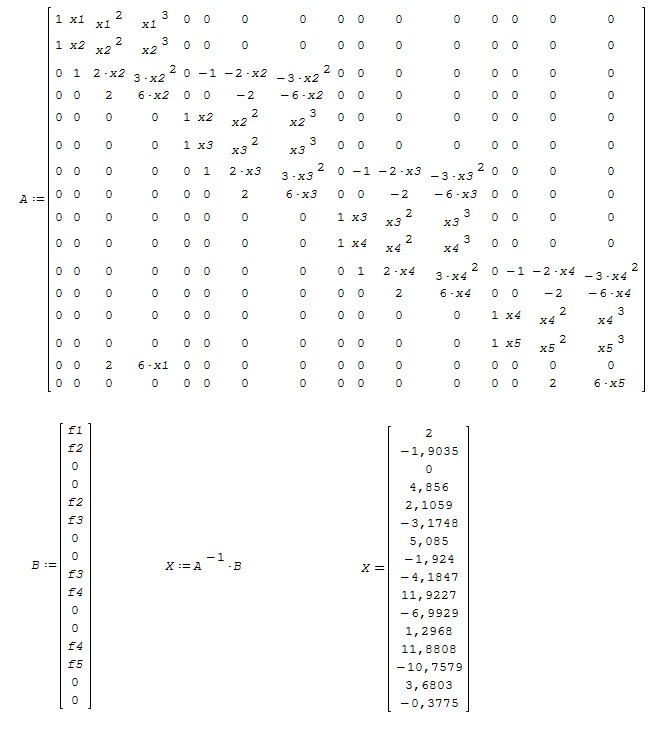
\includegraphics[width=1\linewidth]{matrix.png}} 
\caption{Матрица, составленная из 16 уравнения } \label{matcot}
\end{center}
\end{figure}

Решая уравнение, получаем значение для коэффициэнтов $A_{ij}:

\[
\begin{bmatrix}
A_{10}\\
A_{11}\\
A_{12}\\
A_{13}\\
A_{20}\\
A_{21}\\
A_{22}\\
A_{23}\\
A_{30}\\
A_{31}\\
A_{32}\\
A_{33}\\
\end{bmatrix} = \begin{bmatrix} 2\\ -1.9\\ 0\\ 4.8004\\ 2.1043\\ -3.1517\\ 5.0069\\ -1.8754\\ -3.7168\\ 10.8188\\ -6.1696\\ 1.105\\ 5.5698\\ -2.2916\\ 0\\ 0.1372 \\ 
\end{bmateix}
\]

Окончательно, уравнение для сплайна получаем в виде

\[
F(x)=\begin{cases}
F_1(x)=4.8004 \times x^3+0 \times x^2-1.9 \times x+2 \text{где }x \in [0, 0.25],\\
F_2(x)=-1.8754 \times x^3+5.0069 \times x^2-3.1217 \times x+2.1043 \text{где }x \in [0.25, 1.25],\\
F_3(x)=1.105 \times x^3-6.1696 \times x^2+10.8188 \times x-3.7168 \text{где }x \in [1.25, 2.125],\\
F_4(x)=0.1372 \times x^3+0 \times x^2-2.2916 \times x+5.5698\text{где }x \in [2.125, 3.25].\\
\end{cases}
\] 

По данным уравнениям строим гафик, представленный в соответствии с рисунком \ref{graf6}.

 \begin{figure}[H]
\begin{center}
\begin{tikzpicture}
\begin{scope}[xscale=3, yscale=2]

\draw[thin, ->] (-1,0) -- (3.5,0) node[right] {$X$};
\draw[thin, ->] (0,-1) -- (0,3) node[left] {$Y$};

\draw[domain=0:0.25, smooth, purple] plot ({\x},{4.8004341681*(\x)*(\x)*(\x)+0*(\x)*(\x)-1.900027198*(\x)+2});
\draw[domain=0.25:1.25, smooth, purple] plot ({\x},{-1.87538007721*(\x)*(\x)*(\x)+5.0068619551*(\x)*(\x)-3.1517426868*(\x)+2.1043096241});
\draw[domain=1.25:2.125, smooth, purple] plot ({\x},{1.1050110899*(\x)*(\x)*(\x)-6.169075272*(\x)*(\x)+10.8188441661*(\x)-3.7167682313});
\draw[domain=2.125:3.25, smooth, purple] plot ({\x},{0.137229517*(\x)*(\x)*(\x)+0*(\x)*(\x)-2.2915718292*(\x)+5.569776432});
\filldraw ( 0, 2) circle (0.05cm) node [above,left] {$A(0,2)$};
\filldraw (0.25, 1.6) circle (0.05cm) node [below=15pt,right] {$B(0.25, 1.6)$};
\filldraw (1.25, 2.325) circle (0.05cm) node [above=15pt,right] {$C(1.25, 2.325)$};
\filldraw (2.125, 2.017) circle (0.05cm) node [below=15pt,right] {$D(2.125, 2.017)$};
\filldraw (3.25, 2.833) circle (0.05cm) node [right] {$I(3.25, 2.833)$};
	

\end{scope};
\end{tikzpicture}
\caption{График функции кубического сплайна} \label{graf6}
\end{center}
\end{figure}

\subsection{Вычисление значения функции в точке}

Дальше по заданию необходимо вычислить значение функции при $x=1.2$. Для решения задачи необходимо выбрать функцию, в которой находится данная точка и вместо $x$ подставить её значение. Для решения воспользуемся программой  «SMath studio». Решение представлено в соответствии с рисунком \ref{x1.2}.

\begin{figure}[H]
\begin{center}
\center{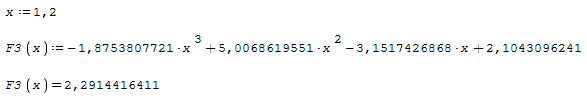
\includegraphics[width=1\linewidth]{x12.png}} 
\caption{Вычисление функции в точке $x=1.2$ } \label{x1.2}
\end{center}
\end{figure}

Полученаа тоска представлена в соответствии с рисунком \ref{graf7}.

 \begin{figure}[H]
\begin{center}
\begin{tikzpicture}
\begin{scope}[xscale=3, yscale=2]

\draw[thin, ->] (-1,0) -- (3.5,0) node[right] {$X$};
\draw[thin, ->] (0,-1) -- (0,3) node[left] {$Y$};

\draw[domain=0:0.25, smooth, purple] plot ({\x},{4.8004341681*(\x)*(\x)*(\x)+0*(\x)*(\x)-1.900027198*(\x)+2});
\draw[domain=0.25:1.25, smooth, purple] plot ({\x},{-1.87538007721*(\x)*(\x)*(\x)+5.0068619551*(\x)*(\x)-3.1517426868*(\x)+2.1043096241});
\draw[domain=1.25:2.125, smooth, purple] plot ({\x},{1.1050110899*(\x)*(\x)*(\x)-6.169075272*(\x)*(\x)+10.8188441661*(\x)-3.7167682313});
\draw[domain=2.125:3.25, smooth, purple] plot ({\x},{0.137229517*(\x)*(\x)*(\x)+0*(\x)*(\x)-2.2915718292*(\x)+5.569776432});
\filldraw ( 0, 2) circle (0.02cm) ;
\filldraw (0.25, 1.6) circle (0.02cm) ;
\filldraw (1.25, 2.325) circle (0.02cm);
\filldraw (2.125, 2.017) circle (0.02cm) ;
\filldraw (3.25, 2.833) circle (0.02cm) ;
\filldraw [red](1.2, 2.2913608) circle (0.03cm) node [above=15pt, right] {$G(1.2, 2.29)$};
		


\end{scope};
\end{tikzpicture}
\caption{Графичекое расположение точки $x=1.2$ на графике функции} \label{graf7}
\end{center}
\end{figure}

\subsection{Определение погрешности функции сплайна в точке}

Для орпеделения погрешности в точке $x_0=2.2$ исползуем формулу \eqref{form1}.

\begin{equation} \label{form1}
R(x_0)=\frac{ \bar{h}^2 \times \left | f^{\prime\prime}(x_0)\right |}{8} - \frac{h_i^2 \times t \times (1-t) \times \left | f^{\prime\prime}(x_0)\right | }{2}
\end{equation} \label{form1}




\section{Задача оптимального распределения неоднородных ресурсов}

Требуется решить следующую задачу оптимального распределения неоднородных ресурсов.

Для изготовления n видов изделий $N_1$,  $N_2$, ... , $N_n$ неходимы ресурсы m видов: трудовые, материальные, финансовые и др.  Известно требуемое количество отдельного i-гo ресурса для изготовления каждого j-го изделия. Назовем эту величину нормой расхода $ c_ {ij}$. Пусть определено количество каждого вида ресурса, которым предприятие располагает в данный момент, – $a_i$. Известна прибыль $Π_i$,  получаемаяпредприятием от изготовления каждого j-го изделия. Требуетсяопределить, какие изделия и в каком количестве должны произво-диться предприятием, чтобы прибыль была максимальной.

Исходные данные представлены в соответствии с рисункои \ref{zadn1}.

\begin{figure}[h!]
\begin{center}
\center{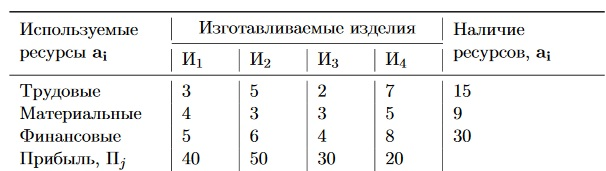
\includegraphics[width=1\linewidth]{3 paint.jpg}} 
\caption{Исходные данные } \label{zadn1}
\end{center}
\end{figure}

Так как данная задача является целочисленной задачей линейного программирования (ILP), стандартная функция мат. пакета «SciLab» . Для решения задачи предназначена функция linpro.

где p  – массив (вектор-столбец) коэффициентов при неизвестных целевой функции, длина вектора n совпадает с количеством неизвестных x;\\
C   –  матрица при неизвестных из левой части системы ограничений,  количество строк матрицы равно количеству ограничений, а количество столбцов совпадает с количеством неизвестных;\\ 
b –  массив (вектор-столбец), содержит свободные члены системы ограничений; \\
ci - массив  (вектор-столбец) содержит нижнюю границу переменных; \\
cs - массив (вектор-столбец) содержит верхнюю границу переменных, если таковая отсутствует,  указывают [ ]. 

Функция linpro возвращает массив неизвестных x, минимальное значение функции f  и массив множителей Лагранжа lagr.

 \\Листинг кода:
\\-->C=[3,5,2,7;4,3,3,5;5,6,4,8;]
\\ C  =
 \\    3.    5.    2.    7.  
    \\4.    3.    3.    5.  
    \\5.    6.    4.    8.  
 \\--> b=[15;9;30;]  
 \\b  =
 \\    15.  
    \\9.   
    \\30.  
\\-->ci=[0;0;0;0;]
 \\ci  =
 \\   0.  
    \\0.  
   \\ 0.  
    \\0.  
 \\-->cs=[]
\\-->p=[40;50;30;20]
 \\p  =
    \\ 40.  
    \\50.  
    \\30.  
    \\20.  
\\ -->[x,lagr,f]=linpro(-p,C,b,ci,cs)
 \\f  =
   - 150.  
 \\x  =
    \\ 0.  
    \\3.  
    \\0.  
    \\0.
  
В результате вычислений утановлено, что максимальную прибыль (150 д. е.) можено получить при производстве изделия № 2. при объёме выпуска 3 ед.

% \begin{figure}[h!]
%\begin{center}
%\begin{tikzpicture}
%\begin{scope}[scale=2]

%\draw[thin, ->] (-1,0) -- (3.5,0) node[right] {$X$};
%\draw[thin, ->] (0,-1) -- (0,4.5) node[left] {$Y$};

%\draw[domain=0:0.25, smooth, purple] plot ({\x},{4.8004341681*(\x)*(\x)*(\x)+0*(\x)*(\x)-1.900027198*(\x)+2});
%\draw[domain=0.25:1.25, smooth, purple] plot ({\x},{-1.87538007721*(\x)*(\x)*(\x)+5.0068619551*(\x)*(\x)-3.1517426868*(\x)+2.1043096241});
%\draw[domain=1.25:2.125, smooth, purple] plot ({\x},{1.1050110899*(\x)*(\x)*(\x)-6.169075272*(\x)*(\x)+10.8188441661*(\x)-3.7167682313});
%\draw[domain=2.125:3.25, smooth, purple] plot ({\x},{0.137229517*(\x)*(\x)*(\x)+0*(\x)*(\x)-2.2915718292*(\x)+5.569776432});
%\filldraw ( 0, 2) circle (0.1cm) node [below=20pt,left=0.1cm] {$A(-3.6652,0)$};
%\filldraw (- 0.5236, 0) circle (0.1cm) node [above=0.5cm,left] {$B(-0.5236, 0)$};
%\filldraw (2.618, 0) circle (0.1cm) node [below=20pt,right] {$C(2.618, 0)$};
%\filldraw (0, 1.5) circle (0.1cm) node [right] {$D(0, 1.5)$};
	
%\end{scope};
%\end{tikzpicture}
%\caption{График функции $h(x)$ в пределах $[0, \frac{5\pi}{6}]} %\label{graf4}
%\end{center}
%\end{figure}

\end{document}